
\caulc
\Opensolutionfile{ans}[ans/ans-01]
\begin{ex}%[1D2H3-4]
	Cho cấp số nhân $(u_n)$ với $u_1=3$ và $u_2=6$. Số hạng $u_6$ của cấp số nhân đã cho bằng
	\choice
	{$21$}
	{$18$}
	{$192$}
	{\True $96$}
	\loigiai{
		Công bội của cấp số nhân là $q=\dfrac{u_2}{u_1}=\dfrac{6}{3}=2$. \\
		Số hạng thứ $6$ là $u_6=u_1 \cdot q^5=3 \cdot 2^5=3 \cdot 32=96$.
	}
\end{ex}

\begin{ex}%[2D4N1-3]
	Họ nguyên hàm của hàm số $f(x)=\sin x-\cos x$ là
	\choice
	{$\cos x+\sin x+C$}
	{$\cos x-\sin x+C$}
	{$-\cos x+\sin x+C$}
	{\True $-\cos x-\sin x+C$}
	\loigiai{
		Ta có $\displaystyle\int (\sin x-\cos x)\mathrm{\,d}x=-\cos x-\sin x+C$.
	}
\end{ex}

\begin{ex}%[2H2N2-2]
	Trong không gian với hệ tọa độ $Oxyz$, cho vectơ $\overrightarrow{v}=(7;6;-4)$. Tọa độ điểm $M$ thỏa mãn $\overrightarrow{OM}=\overrightarrow{v}$ là
	\choice
	{$(7;-6;4)$}
	{$(7;0;-4)$}
	{\True $(7;6;-4)$}
	{$(-7;-6;-4)$}
	\loigiai{
		Vì $\overrightarrow{OM}=(x_M;y_M;z_M)$ nên $\overrightarrow{OM}=\overrightarrow{v}=(7;6;-4) \Rightarrow M(7;6;-4)$.
	}
\end{ex}

\begin{ex}%[2H2H1-2]
	\immini{Cho hình lập phương $ABCD.EFGH$ có độ dài cạnh bằng $4a$. Độ dài của vectơ $\overrightarrow{x}=\overrightarrow{EF}+\overrightarrow{EH}$ bằng}{\begin{tikzpicture}[scale=0.7, font=\footnotesize, line join=round, line cap=round, >=stealth, declare function={bc=4; ba=2; h=3; gocnghieng=90; gocB=35;}]
			\path
			(0,0) coordinate (B)
			(gocB:ba) coordinate (A)
			(bc,0) coordinate (C)
			($(C)-(B)+(A)$) coordinate (D)
			($(A)+(gocnghieng:h)$) coordinate (E)
			($(B)-(A)+(E)$) coordinate (F)
			($(C)-(A)+(E)$) coordinate (G)
			($(D)-(A)+(E)$) coordinate (H);
			\draw
			(F)--(B)--(C)--(D)--(H)--(E)--(F)--(G)--(H)
			(C)--(G);
			\draw[dashed]
			(E)--(A)--(D)
			(A)--(B);
			\foreach \diem/\goc in {
				A/135, B/-135, C/-45, D/45,
				E/135, F/180, G/-45, H/45
			}
			\fill[black] (\diem) circle (1.5pt) ++(\goc:0.35) node{$\diem$};
	\end{tikzpicture}}
	\choice
	{$4\sqrt{3}a$}
	{$8a$}
	{$24a$}
	{\True $4\sqrt{2}a$}
	\loigiai{
		Theo quy tắc hình bình hành, ta có $\overrightarrow{EF}+\overrightarrow{EH}=\overrightarrow{EG}$. \\
		Suy ra độ dài $\left|\overrightarrow{x}\right|=EG=\sqrt{EF^2+FG^2}=\sqrt{(4a)^2+(4a)^2}=4\sqrt{2}a$.
	}
\end{ex}

\begin{ex}%[2D1N4-1]
	Đường tiệm cận đứng của đồ thị hàm số $y=\dfrac{2x-1}{x-1}$ có phương trình là
	\choice
	{$y=2$}
	{\True $x=1$}
	{$y=1$}
	{$x=-1$}
	\loigiai{
		Ta có $\displaystyle\lim\limits_{x\to 1^+}y=\displaystyle\lim\limits_{x\to 1^+}\dfrac{2x-1}{x-1}=+\infty$ và $\displaystyle\lim\limits_{x\to 1^-}y=\displaystyle\lim\limits_{x\to 1^-}\dfrac{2x-1}{x-1}=-\infty$.\\
		Suy ra đồ thị hàm số đã cho có tiệm cận đứng là $x=1$.
	}
\end{ex}

\begin{ex}%[1D1H5-3]
	Tập nghiệm của phương trình $2\cos x-1=0$ là
	\choice
	{$S=\left\{-\dfrac{\pi}{3}+k2\pi\middle| k \in \mathbb{Z}\right\}$}
	{\True $S=\left\{\dfrac{\pi}{3}+k2\pi;-\dfrac{\pi}{3}+k2\pi\middle| k \in \mathbb{Z}\right\}$}
	{$S=\left\{\dfrac{\pi}{3}+k2\pi\middle| k \in \mathbb{Z}\right\}$}
	{$S=\left\{\dfrac{\pi}{3}+k\pi\middle| k \in \mathbb{Z}\right\}$}
	\loigiai{
	Ta có $2\cos x-1=0 \Leftrightarrow \cos x=\dfrac{1}{2}=\cos \dfrac{\pi}{3} \Leftrightarrow x=\pm\dfrac{\pi}{3}+k2\pi$, với $k\in \mathbb{Z}$.
	}
\end{ex}

\begin{ex}%[1D6H4-3]
	Tập nghiệm của bất phương trình $\log_{0{,}5}(x-1)>1$ là
	\choice
	{$\left(-\infty;\dfrac{3}{2}\right)$}
	{$\left(\dfrac{3}{2};+\infty\right)$}
	{$\left[1;\dfrac{3}{2}\right)$}
	{\True $\left(1;\dfrac{3}{2}\right)$}
	\loigiai{
		Điều kiện xác định $x-1>0 \Leftrightarrow x>1$. \\
		Ta có $\log_{0{,}5}(x-1)>1 \Leftrightarrow x-1<0{,}5^1 \Leftrightarrow x<\dfrac{3}{2}$. \\
		Kết hợp điều kiện ta được $1<x<\dfrac{3}{2}$.\\
		Vậy tập nghiệm của bất phương trình là $S=\left(1;\dfrac{3}{2}\right)$.
	}
\end{ex}

\begin{ex}%[2D3N1-3]
	Cho mẫu số liệu ghép nhóm về cân nặng (đơn vị: kg):
	\begin{center}
		\begin{tabular}{|c|c|c|c|c|c|c|}
			\hline
			Cân nặng & $[45;50)$ & $[50;55)$ & $[55;60)$ & $[60;65)$ & $[65;70)$ & $[70;75)$ \\
			\hline
			Số người & $12$ & $4$ & $16$ & $31$ & $13$ & $20$ \\
			\hline
		\end{tabular}
	\end{center}
	Trung vị của mẫu số liệu trên bằng
	\choice
	{$67{,}58$}
	{$72{,}90$}
	{$52{,}58$}
	{\True $62{,}58$}
	\loigiai{
		Cỡ mẫu $n=96$. Và $\dfrac{n}{2}=48$. Suy ra nhóm chứa trung vị là $[60;65)$. \\
		Khi đó trung vị của mẫu số liệu đã cho là $M_e=60+\dfrac{48-32}{31} \cdot 5 \approx 62{,}58$.
	}
\end{ex}

\begin{ex}%[1H8H7-4]
	\immini{Cho khối lăng trụ đứng $ABC.A'B'C'$ có $AA'=5$, $AB=2$, $AC=3$ và tam giác $ABC$ vuông tại $A$. Thể tích khối lăng trụ bằng}{\begin{tikzpicture}[scale=0.65, font=\footnotesize, line join=round, line cap=round, >=stealth, declare function={ac=4; ab=2; h=3.5; gocA=35;}]
			\path
			(0,0) coordinate (A)
			(ac,0) coordinate (C)
			(-gocA:ab) coordinate (B)
			($(A)+(90:h)$) coordinate (A')
			($(B)-(A)+(A')$) coordinate (B')
			($(C)-(A)+(A')$) coordinate (C');
			\draw
			(A')--(A)--(B)--(C)--(C')--(A')--(B')--(C') (B)--(B');
			\draw[dashed] (A)--(C);
			\foreach \diem/\goc in {A/-135, B/-90, C/-45, A'/135, B'/80, C'/45}
			\fill[black] (\diem) circle (1.5pt) ++(\goc:0.4) node{$\diem$};
	\end{tikzpicture}}
	\choice
	{$5$}
	{$30$}
	{\True $15$}
	{$10$}
	\loigiai{
		Diện tích đáy $S_{ABC}=\dfrac{1}{2} \cdot 2 \cdot 3=3$. \\
		Thể tích khối lăng trụ đã cho là $V=S_{ABC}\cdot AA'=3 \cdot 5=15$ (đvtt).
	}
\end{ex}

\begin{ex}%[2D4N3-1]
	Diện tích $S$ của hình phẳng giới hạn bởi đồ thị $y=3x-4$, trục hoành và hai đường thẳng $x=1,x=2$ được xác định bằng công thức
	\choice
	{\True $S=\displaystyle\int\limits_1^2 |3x-4| \mathrm{\,d}x$}
	{$S=\pi\displaystyle\int\limits_1^2 |3x-4|\mathrm{\,d}x$}
	{$S=\pi\displaystyle\int\limits_1^2 (3x-4)^2\mathrm{\,d}x$}
	{$S=\left|\displaystyle\int\limits_1^2 (3x-4)\mathrm{\,d}x\right|$}
	\loigiai{
	Diện tích $S$ của hình phẳng giới hạn bởi đồ thị $y=3x-4$, trục hoành và hai đường thẳng $x=1,x=2$ là $S=\displaystyle\int\limits_1^2 |3x-4| \mathrm{\,d}x$	
	}
\end{ex}

\begin{ex}%[1H4N3-2]
	Cho hình chóp $S.ABCD$ có đáy $ABCD$ là hình bình hành. Đường thẳng $AB$ song song với mặt phẳng nào sau đây?
	\choice
	{$(SAC)$}
	{\True $(SCD)$}
	{$(SBD)$}
	{$(SBC)$}
	\loigiai{
		Vì $AB \parallel CD$ và $CD \subset (SCD)$ nên $AB \parallel (SCD)$.
	}
\end{ex}

\begin{ex}%[2H5N2-1]
	Trong không gian với hệ tọa độ $Oxyz$, đường thẳng $\Delta\colon\heva{&x=-1+t \\ &y=7+7t \\ &z=7+5t}$ đi qua điểm nào trong các điểm sau?
	\choice
	{\True $P(1;21;17)$}
	{$M(3;20;-5)$}
	{$N(1;-7;-7)$}
	{$Q(1;7;5)$}
	\loigiai{
		Thay tọa độ $P(1;21;17)$ vào hệ phương trình
		$\heva{&1=-1+t \\ &21=7+7t \\ &17=7+5t} \Leftrightarrow \heva{&t=2 \\ &t=2 \\ &t=2}$.\\
		Vậy đường thẳng đi qua $P$.
	}
\end{ex}

\Closesolutionfile{ans}

\cauds

\Opensolutionfile{ans}[ans/answer]
\begin{ex}%[2D6H1-4]
	Trước khi tung ra một dòng điện thoại mới, một công ty tiến hành phỏng vấn ngẫu nhiên $250$ khách hàng. Kết quả thống kê như sau: có $120$ người trả lời \lq\lq sẽ mua\rq\rq; có $130$ người trả lời \lq\lq không mua\rq\rq. Kinh nghiệm cho thấy tỉ lệ khách hàng thực sự sẽ mua sản phẩm đối với những người trả lời \lq\lq sẽ mua\rq\rq \, và \lq\lq không mua\rq\rq \, tương ứng là $80\%$ và $20\%$.
	Gọi $A$ là biến cố \lq\lq Người được phỏng vấn thực sự sẽ mua sản phẩm\rq\rq.
	Gọi $B$ là biến cố \lq\lq Người được phỏng vấn trả lời sẽ mua sản phẩm\rq\rq.
	\choiceTF
	{$\mathrm{P}(\overline{B})=0{,}48$}
	{\True $\mathrm{P}(A|B)=0{,}8$}
	{$\mathrm{P}(A)=0{,}38$}
	{Trong số những người được phỏng vấn thực sự sẽ mua sản phẩm, có $70\%$ người đã trả lời \lq\lq sẽ mua\rq\rq \, khi được phỏng vấn (\textit{kết quả tính theo phần trăm được làm tròn đến hàng đơn vị})}
	\loigiai{
		\begin{itemchoice}
			\itemch Ta có $\mathrm{P}(B)=\dfrac{120}{250}=0{,}48$; $\mathrm{P}(\overline{B})=\dfrac{130}{250}=0{,}52$.
			\itemch Và $\mathrm{P}(A|B)=0{,}8$.
			\itemch Ta lại có $\mathrm{P}(A)=\mathrm{P}(B)\mathrm{P}(A|B)+\mathrm{P}(\overline{B})\mathrm{P}(A|\overline{B})=0{,}48 \cdot 0{,}8+0{,}52 \cdot 0{,}2=0{,}488$. 
			\itemch Và $\mathrm{P}(B|A)=\dfrac{\mathrm{P}(B)\mathrm{P}(A|B)}{\mathrm{P}(A)}=\dfrac{0{,}384}{0{,}488} \approx 79\%$.
		\end{itemchoice}
	}
\end{ex}

\begin{ex}%[1D3V2-8]
	Một thùng trộn tại một nhà máy sản xuất kem hiện chứa $2\,000$ lít nước, trong đó có $5$ kg đường đã được trộn. Một vòi nước sẽ được mở với tốc độ $50$ lít mỗi phút vào thùng, cùng lúc đường được đổ vào thùng với tốc độ $1$ kg mỗi phút.
	\choiceTF
	{\True Khối lượng đường trong thùng trộn sau $t$ phút là $1\,000t+5\,000$ (gam)}
	{\True Nồng độ đường trong thùng sau $t$ phút (đơn vị gam/lít) là $f(t)=\dfrac{1\,000t+5\,000}{50t+2\,000}$}
	{\True Xem $y=f(t)$ là một hàm số xác định trên $[0;+\infty)$ thì nồng độ đường trong thùng luôn tăng khi sản xuất trong thời gian dài liên tục}
	{Với tiêu chuẩn nồng độ không quá $20$ gam/lít, nhà máy không thể sản xuất liên tục trong một thời gian dài}
	\loigiai{
		\begin{itemchoice}
			\itemch Khối lượng đường trong thùng trộn sau $t$ phút là $1\,000t+5\,000$ (gam).
			\itemch Thể tích nước trong thùng sau thời gian $t$ phút là $50t+2\,000$.\\
			Do đó nồng độ đường trong thùng sau $t$ phút là $f(t)=\dfrac{1\,000t+5\,000}{50t+2\,000}$.
			\itemch Ta có $f'(t)=\dfrac{1750}{(50t+2\,000)^2}$. Vì $f'(t) > 0$ trên $[0;+\infty)$ nên hàm số $f(t)$ đồng biến trên $[0;+\infty)$.\\
			Do đó ta có thể khẳng định nồng độ đường trong thùng luôn tăng khi sản xuất trong thời gian liên tục.
			\itemch Do $\lim\limits_{x \to +\infty} f(t)=\lim\limits_{t \to +\infty} \dfrac{1\,000t+5\,000}{50t+2\,000}=20$ và $f'(t)>0$ nên ta có $f(t) < 20$ với mọi giá trị $t \ge 0$. Tức là nhà máy có thể sản xuất liên tục trong một thời gian dài.
		\end{itemchoice}
	}
\end{ex}

\begin{ex}%[2D1H5-6]
	Cho hàm số $y=f(x)=\dfrac{x^2+x-1}{x+2}$.
	\choiceTF
	{\True Tập xác định của hàm số $y=f(x)$ là $\mathbb{R} \setminus \{-2\}$}
	{\True Đồ thị hàm số $y=f(x)$ có hai điểm cực trị nằm cùng phía với trục hoành}
	{Tâm đối xứng của đồ thị hàm số $y=f(x)$ là điểm $I(2;1)$}
	{\True Gọi $M$ là giao điểm của đồ thị với trục tung. Tiếp tuyến của đồ thị tại $M$ là $y=\dfrac{3}{4}x-\dfrac{1}{2}$}
	\loigiai{
		\begin{itemchoice}
			\itemch Điều kiện xác định $x+2\ne 0\Rightarrow x\ne -2$. Suy ra tập xác định của hàm số $y=f(x)$ là $\mathbb{R} \setminus \{-2\}$.
			\itemch Ta có $y'=\dfrac{x^2+4x+3}{(x+2)^2}$. Cho $y'=0\Rightarrow x^2+4x+3=0 \Rightarrow \hoac{&x=-1\\&x=-3}$. \\
			Suy ra hai điểm cực trị của đồ thị hàm số là $A(-1;-1)$, $B(-3;-5)$. Và hai điểm $A$, $B$ nằm về cùng một phía với trục hoành.
			\itemch Ta có $\displaystyle\lim\limits_{x\to (-2)^+}f(x)=\displaystyle\lim\limits_{x\to (-2)^+}\dfrac{x^2+x-1}{x+2}=+\infty$ và $\displaystyle\lim\limits_{x\to (-2)^-}f(x)=\displaystyle\lim\limits_{x\to (-2)^-}\dfrac{x^2+x-1}{x+2}=-\infty$ hay $x=-2$ là tiệm cận đứng của đồ thị hàm số $y=f(x)$.\\
			Ta lại có $\displaystyle\lim\limits_{x\to \pm\infty}\left( f(x)-x+1\right) =\displaystyle\lim\limits_{x\to \pm \infty}\left(\dfrac{x^2+x-1}{x+2}-x+1\right)=0$ hay $y=x-1$ là tiệm cận xiên của đồ thị hàm số $y=f(x)$.\\
			Suy ra tâm đối xứng của đồ thị hàm số $y=f(x)$ là $I(-2;-3)$.
			\itemch Thế $x=0$ vào $y=f(x)=\dfrac{x^2+x-1}{x+2}$ ta được $y=-\dfrac{1}{2}$, suy ra $M\left(0;-\dfrac{1}{2}\right)$ và $f'(0)=\dfrac{3}{4}$.\\
			Phương trình tiếp tuyến của đồ thị hàm số $y=f(x)$ tại $M\left(0;-\dfrac{1}{2}\right)$ là 
			\[y=\dfrac{3}{4}(x-0)-\dfrac{1}{2}=\dfrac{3}{4}x-\dfrac{1}{2}.\]
		\end{itemchoice}	
	}
\end{ex}

\begin{ex}%[2H5V3-4]
	Trong không gian $Oxyz$, mặt cầu $(S)$ có phương trình $(x-2)^2+(y+1)^2+(z+1)^2=6$. Một tấm gỗ mỏng tiếp xúc với bề mặt quả bóng, phần giao của tấm gỗ và sàn nhà là đường thẳng $d\colon\dfrac{x+2}{2}=\dfrac{y+1}{-3}=\dfrac{z}{1}$. Gọi $A$, $B$ tương ứng là tiếp điểm của tấm gỗ, sàn nhà với quả bóng.
	\choiceTF
	{\True Mặt cầu $(S)$ có bán kính $R=\sqrt{6}$ và tâm $I(2;-1;-1)$}
	{Nếu $K$ là một điểm thuộc đường thẳng $d$ thì $K(-2+2t;-1-3t;-t)$ với $t \in \mathbb{R}$}
	{\True Hình chiếu của tâm $I$ lên đường thẳng $d$ là điểm $K$ có tọa độ $(a;b;c)$ thỏa mãn $b+c<0$}
	{Một con kiến bò trên bề mặt quả bóng từ $A$ đến $B$ thì quãng đường ngắn nhất lớn hơn $45$ cm}
	\loigiai{
		\begin{itemchoice}
			\itemch Quả bóng có tâm $I(2;-1;-1)$ và bán kính $R=\sqrt{6}$.
			\itemch Đường thẳng $d$ đi qua điểm $M(-2;-1;0)$ và có vectơ chỉ phương $\overrightarrow{u}=(2;-3;1)$ nên có phương trình tham số là $\heva{&x=-2+2t\\&y=-1-3t\\&z=t}$.\\
			Nếu $K$ là một điểm thuộc đường thẳng $d$ thì $K(-2+2t;-1-3t;t)$.
			\itemch Gọi $K$ là hình chiếu vuông góc của $I$ lên $d$, suy ra $K(-2+2t;-1-3t;t)$.\\
			Ta có $\overrightarrow{IK}=(2t-4;-3t;t+1)$.\\
			Khi đó $\overrightarrow{IK} \cdot \vec{u}=0\Leftrightarrow 4t-8+9t+t+1=0\Rightarrow t=\dfrac{1}{2}$ nên suy ra $K\left(-1;-\dfrac{5}{2};\dfrac{1}{2}\right)$.\\
			Hay $b+c=-\dfrac{5}{2}+\dfrac{1}{2}=-2<0$.
			\itemch Hình vẽ
			\begin{center}
				\begin{tikzpicture}[line join=round, line cap=round, >=stealth, font=\footnotesize, scale=1, declare function={R=2; d=3.5;}]
					\path
					(-3.5,1) coordinate (E)
					(0,0) coordinate (I)
					(180:d) coordinate (K)
					($(E)!3!(K)$) coordinate (F)
					;
					\draw[name path=dtO, ] (I) circle (R);
					\path[name path=dtI] ($(K)!0.5!(I)$) circle (0.5*d);
					\path[name intersections={of= dtO and dtI}] coordinate (A) at (intersection-1) coordinate (B) at (intersection-2);    
					\draw (K)--(I)--(A)--(K)--(B)--(I) (E)--(F)node[right]{$d$};
					\foreach \mot/\hai/\ba in {K/A/I, K/B/I,F/K/I}
					\draw pic[draw=black,angle radius=4pt] {right angle=\mot--\hai--\ba};
					\foreach \diem/\goc in {K/180, I/0, A/90, B/-90} 
					\fill (\diem) circle (1.5pt) ++(\goc:0.25) node{$\diem$};  
				\end{tikzpicture}
			\end{center}
			Ta có $\overrightarrow{IK}=\left(-3;-\dfrac{3}{2};\dfrac{3}{2}\right)\Rightarrow IK=\dfrac{3\sqrt{6}}{2}$ nên $\cos \widehat{AIK}= \dfrac{IA}{IK}=\dfrac{2}{3}$, suy ra $\cos \widehat{AIB}=-\dfrac{1}{9}$.\\
			Suy ra $\widehat{AIB}\approx 96{,}38^\circ=n^\circ$.\\
			Độ dài cung tròn bé nhất là $l=\dfrac{\pi \cdot R\cdot n}{180}\approx 41{,}2$ cm.
		\end{itemchoice}
	}
\end{ex}

\Closesolutionfile{ans}

\caukq
\setcounter{ex}{0}

\Opensolutionfile{ans}[ans-KQ]

\begin{ex}%[1H8V7-6]
\immini{Một thùng đựng rác có dạng hình chóp cụt đều. Đáy và miệng thùng là các hình vuông tương ứng có độ dài cạnh bằng $60$ cm và $120$ cm, cạnh bên của thùng dài $100$ cm. Thể tích của thùng đựng rác đã cho bằng bao nhiêu đề-xi-mét khối (\textit{không làm tròn kết quả các phép tính trung gian, chỉ làm tròn kết quả cuối cùng đến hàng đơn vị})?}{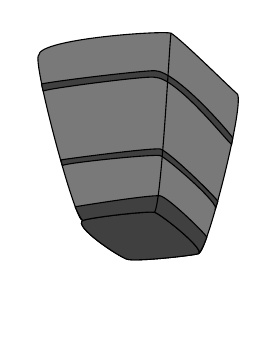
\begin{tikzpicture}[line join=round, line cap=round,scale=0.7,transform shape]
		\clip (2,-3) rectangle (6,2.5);
		\tikzset{binh/.pic={
				\def\A{
					(-5.1,1.6)
					..controls +(20:.1) and +(160:.15) ..(-3.8,1.7)
					..controls +(-20:.2) and +(30:.2) ..(-3,1)
					..controls +(30:.15) and +(30:.15) ..(-2.2,-2)
					..controls +(-90:.3) and +(-20:.15) ..(-4.6,-2.4)
					..controls +(150:.2) and +(-40:.15) ..(-5.8,-1.3)
					..controls +(140:.2) and +(180:.15) ..cycle
					;
				}
				\fill[darkgray!70] \A;
				\draw[black]\A;
				\def\D{
					(-5.1,1.6)
					..controls +(20:.1) and +(160:.15) ..(-3.8,1.7)
					..controls +(-20:.2) and +(30:.2) ..(-3,1)
					..controls +(-150:.1) and +(-10:.15) ..(-4.3,.85)
					..controls +(170:.1) and +(-150:.15) ..cycle
					;
				}
				\fill[darkgray] \D;
				\draw[black]\D;
				\draw[fill=darkgray] (-3,1)
				..controls +(-150:.1) and +(-10:.15) ..(-4.3,.85)
				..controls +(170:.1) and +(-150:.15) ..(-5.1,1.6)
				..controls +(-130:.1) and +(70:.15) ..(-5.25,1.3)
				..controls +(-60:.1) and +(170:.15) ..(-4.4,.55)
				..controls +(-5:.2) and +(-170:.15) ..(-2.86,.75)
				..controls +(120:.05) and +(-30:.05) ..cycle
				(-2.63,0)
				..controls +(-150:.1) and +(-10:.15) ..(-4.4,-.18)
				..controls +(170:.1) and +(-150:.15) ..(-5.4,.8)--(-5.45,.65)
				..controls +(-60:.1) and +(170:.15) ..(-4.4,-.3)
				..controls +(-5:.2) and +(-170:.15) ..(-2.6,-.1)--cycle
				(-2.28,-1.35)
				..controls +(-150:.1) and +(-20:.1) ..(-4.3,-1.6)
				..controls +(180:.4) and +(-40:.15) ..(-5.7,-.38)--(-5.72,-.5)
				..controls +(-60:.1) and +(180:.4) ..(-4.3,-1.72)
				..controls +(0:.2) and +(-170:.5) ..(-2.25,-1.48)--cycle
				;
				\draw (-4.3,.85) ..controls +(-130:.2) and +(80:.15) ..(-4.6,-2.4);
		}}
		\path
		(0,0)pic[scale=1,rotate=180]{binh}
		;
\end{tikzpicture}}
	\par \shortans[oly]{761}
	\loigiai{
		Gọi thùng đựng rác là hình chóp cụt đều $ABCD.A'B'C'D'$ và ta xét một mặt chéo của thùng đựng rác như hình vẽ bên dưới
		\begin{center}
			\begin{tikzpicture}[line join = round, line cap = round,>=stealth,font=\footnotesize,scale=0.8,declare function={b=3;a=4.75;h=3.5;}]
				\path
				(0,0) coordinate (A)
				($(A)+(b,0)$) coordinate (C)
				($(A)+(-1.5,h)$) coordinate (A')
				($(C)+(1.5,h)$) coordinate (C')
				($(A')!(A)!(C')$) coordinate (H) %chân đường cao
				;
				\draw (A)--(C)--(C')--(A')--cycle (A)--(H);
				\draw pic[draw=black,angle radius=4pt] {right angle = A'--H--A};
				\foreach \diem/\goc in {A/-90, C/-90, A'/120, C'/60,H/90}
				\fill[black] (\diem) circle (1pt) ++(\goc:0.25) node{$\diem$};
				\draw [<->] (0,-0.5)--(3,-0.5) node[midway,sloped,below]{$6$ dm};
				\draw [<->] (-1.5,4)--(4.5,4) node[midway,sloped,above]{$12$ dm};
				\draw [<->] ($(A)+(-0.5,0)$)--($(A')+(-0.5,0)$) node[midway,sloped,below]{$10$ dm};
			\end{tikzpicture}
		\end{center}
		Gọi $H$ là hình chiếu vuông góc của $A$ lên $A'C'$, suy ra $AH$ chính là chiều cao của thùng đựng rác và $A'H=\dfrac{A'C'-AC}{2}=3\sqrt{2}$ (dm).\\
		Xét $\Delta AHA'$ vuông tại $H$, ta có 
		\[AH^2=AA'^2-A'H^2=100-18=82\Rightarrow AH=\sqrt{82}\, \text{(dm)}.\]
		Thể tích của thùng đựng rác là
		\[V=\dfrac{1}{3}\left(12^2+6^2+\sqrt{12^2\cdot 6^2}\right)\cdot \sqrt{82}\approx 761 \, (\text{dm}^3).\]
	}
\end{ex}

\begin{ex}%[0D8V1-3]
	Người ta muốn lát kín một bảng ô vuông kích thước $3 \times 13$ ($3$ hàng $13$ cột) bằng các tấm bìa kích thước $1 \times 2$ và $1 \times 3$ sao cho các tấm bìa không được chồng lên nhau hay phủ ra ngoài bảng. Có bao nhiêu cách lát nếu ta được phép xoay các tấm bìa nhưng cạnh dài của tất cả các tấm bìa đều phải song song với nhau (số lượng mỗi loại tấm bìa không hạn chế)?
	\begin{center}
		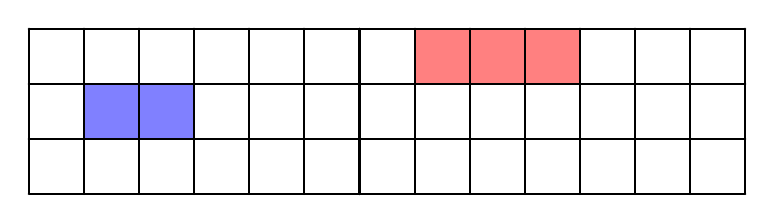
\begin{tikzpicture}[line cap=round, line join=round, >=stealth, font=\footnotesize,scale=0.7]
			\fill [blue!50] (1,1) rectangle (3,2);
			\fill [red!50] (7,2) rectangle (10,3);
			\draw[thick] (0,0) grid[step=1cm] (13,3);
		\end{tikzpicture}
	\end{center}
	\par \shortans[oly]{4097}
	\loigiai{
		Theo giả thiết ta xét $2$ trường hợp.\\
		\textbf{Trường hợp 1:} Các tấm bìa đều xếp thẳng đứng.\\
		Như vậy chỉ có thể dùng các tấm $1 \times 3$. Và trường hợp này chỉ có đúng một cách lát.\\
		\textbf{Trường hợp 2:} Các tấm bìa đều xếp nằm ngang.\\
		Trước hết ta đếm số cách lát một hàng ngang gồm $13$ ô vuông.\\
		Gọi $x$ là số tấm có độ dài là $2$ và $y$ là số tấm có độ dài là $3$ thì ta có $2x+3y=13$.\\
		Ta thấy phương trình có hai nghiệm nguyên không âm là $(x;y)=(2;3)$ và $(x;y)=(5;1)$.
		\begin{itemize}
			\item Với trường hợp $(x;y)=(2;3)$ ta có $5$ tấm và mỗi cách lát sẽ xác định duy nhất bởi thứ tự các tấm trên hàng ngang. Như vậy trong trường hợp này số cách lát bằng số cách chọn ra $2$ vị trí trong $5$ vị trí để đặt tấm $1 \times 2$. Do đó có $\mathrm{C}_5^2=10$ cách.
			\item Tương tự trường hợp $(x;y)=(5;1)$ ta có $6$ tấm và mỗi cách lát sẽ xác định duy nhất bởi thứ tự các tấm trên hàng ngang. Như vậy trong trường hợp này số cách lát bằng số cách chọn ra $1$ vị trí trong $6$ vị trí để đặt tấm $1 \times 3$. Do đó có $\mathrm{C}_6^1=6$ cách.
		\end{itemize}
		Tổng cộng ta có $16$ cách lát một hàng ngang. Do đó theo quy tắc nhân trong trường hợp $2$ ta có $16^3 = 4\,096$ cách lát.\\
		Vậy có $1+4\,096=4\,097$ cách lát thỏa yêu cầu.
	}
\end{ex}

\begin{ex}%[2D4V3-2]
	Cho hai hàm số $y=f(x)=ax^3+bx^2+cx-2$ và $y=g(x)=dx^2+ex+2$ ($a$, $b$, $c$, $d$, $e \in \mathbb{R}$). Biết rằng đồ thị của hàm số $y=f(x)$ và $y=g(x)$ cắt nhau tại ba điểm có hoành độ lần lượt là $-2$; $-1$; $1$. Hình phẳng giới hạn bởi hai đồ thị đã cho có diện tích bằng bao nhiêu (\textit{không làm tròn kết quả các phép tính trung gian, chỉ làm tròn kết quả cuối cùng đến hàng phần mười})?
	\begin{center}
		\begin{tikzpicture}[scale=0.8, font=\footnotesize, line join=round, line cap=round,>=stealth]
			\def\xmax{3} \def\ymax{3.5}			
			\draw[->] (-2.5,0)--(\xmax,0) node [below]{$x$};
			\draw[->] (0,-4)--(0,\ymax) node [left]{$y$};
			\fill (0,0) circle(1.5pt) node[below left]{$O$};
			\draw[thick,blue,samples=100,smooth,domain=-2.15:1.15,variable=\x] plot (\x,{2*(\x)^3+3*(\x)^2-3/2*(\x)-2})node[right]{$y=f(x)$};
			\draw[thick,red,samples=100,smooth,domain=-2.3:1.3,variable=\x] plot (\x,{-1*(\x)^2+1/2*(\x)+2})node[right]{$y=g(x)$};
			\fill [color=gray!200,pattern=north east lines,pattern color=blue, variable=\x] plot[domain=-2:1](\x,{2*(\x)^3+3*(\x)^2-3/2*(\x)-2})--plot[domain=1:-2](\x,{-1*(\x)^2+1/2*(\x)+2});
			\draw[dashed] (-2,-3)--(-2,0)node[above]{$-2$} (-1,0.5)--(-1,0)node[below]{$-1$} (1,1.5)--(1,0)node[below]{$1$};
		\end{tikzpicture}
	\end{center}
	\par \shortans[oly]{6,2}
	\loigiai{
		Phương trình hoành độ giao điểm của đồ thị $f(x)$ và $g(x)$ là
		\[ax^3+bx^2+cx-2=dx^2+3x+2 \Leftrightarrow ax^3+(b-d)x^2+(c-e)x-4=0. \quad (*)\]
		Do đồ thị của hai hàm số cắt nhau tại ba điểm suy ra phương trình $(*)$ có ba nghiệm $x=-2$; $x=-1$; $x=1$. Ta được
		\[ax^3+(b-d)x^2+(c-e)x-4 = k(x+2)(x+1)(x-1).\]
		Khi đó $-4=-2k \Rightarrow k=2$.\\
		Vậy diện tích hình phẳng cần tìm là $\displaystyle\int\limits_{-2}^1 \left|2(x+2)(x+1)(x-1)\right|\mathrm{\,d}x = \dfrac{37}{6} \approx 6{,}2$ (đvdt).
	}
\end{ex}

\begin{ex}%[0D0V2-6]
	Một bảng hình vuông kích thước $10 \times 10$ gồm 100 hình vuông đơn vị, mỗi hình vuông đơn vị có diện tích bằng $1$ (tham khảo hình vẽ). Chọn ngẫu nhiên một hình chữ nhật tạo thành từ các hình vuông đơn vị của bảng. Xác suất để hình chữ nhật chọn được có diện tích là một số chẵn bằng $\dfrac{a}{b}$ với $\dfrac{a}{b}$ là phân số tối giản. Khi đó giá trị của $P=a+b$ bằng bao nhiêu?
	\begin{center}
		
\begin{tikzpicture}[line cap=round, line join=round, >=stealth, font=\footnotesize,scale=0.7]
		\draw[thick] (0,0) grid[step=0.5cm] (5,5);
		\end{tikzpicture}
	\end{center}
	\par \shortans[oly]{206}
	\loigiai{
		Mỗi hình chữ nhật được tạo thành bằng cách chọn $2$ đường nằm ngang (từ $11$ đường) và $2$ đường nằm dọc (từ $11$ đường).\\
		Số hình chữ nhật là: $n\left(\Omega\right)=\mathrm{C}_{11}^2 \cdot \mathrm{C}_{11}^2=3\,025$.\\
		Gọi $A$ là biến cố "chọn được hình chữ nhật có diện tích chẵn".\\
		Biến cố đối $\overline{A}$ là "chọn được hình chữ nhật có diện tích lẻ".\\
		Để diện tích hình chữ nhật là số lẻ thì cả hai kích thước (chiều dài và chiều rộng) của nó đều phải là số lẻ.\\
		Đánh số các đường nằm ngang từ $1$ đến $11$, các đường thẳng đứng từ $1$ đến $11$.\\
		Khi đó, theo mỗi phương có $6$ đường số lẻ $\{1,3,5,7,9,11\}$ và $5$ đường số chẵn $\{2,4,6,8,10\}$.
		\begin{itemize}
			\item Để tạo ra một cạnh có độ dài lẻ, ta phải chọn $1$ đường lẻ và $1$ đường chẵn.
			\item Số cách chọn kích thước thứ nhất là lẻ, có $6 \cdot 5=30$ cách.
			\item Số cách chọn kích thước thứ hai là lẻ, có $6 \cdot 5=30$ cách.
		\end{itemize}
		Suy ra $n\left(\overline{A}\right)=30 \cdot 30=900$.\\
		Khi đó $\mathrm{P}\left(\overline{A}\right)=\dfrac{900}{3\,025}=\dfrac{36}{121}$.
		Suy ra $\mathrm{P}(A)=1-\mathrm{P}\left(\overline{A}\right)=1-\dfrac{36}{121} = \dfrac{85}{121}$.\\
		Vậy $a=85$, $b=121$ hay $a+b=206$.
	}
\end{ex}

\begin{ex}%[2D1V3-6]
	Từ một tấm bìa lục giác đều cạnh bằng $20$, bạn Bình muốn làm một hình chóp lục giác đều bằng cách cắt bỏ phần tô đậm và dán các mép lại với nhau (các mối ghép nối có kích thước không đáng kể, tham khảo hình vẽ). Để thể tích khối chóp lục giác đều tạo thành lớn nhất thì phần diện tích bạn Bình cắt đi là bao nhiêu (\textit{không làm tròn kết quả các phép tính trung gian, chỉ làm tròn kết quả cuối cùng đến hàng đơn vị})?
\begin{center}
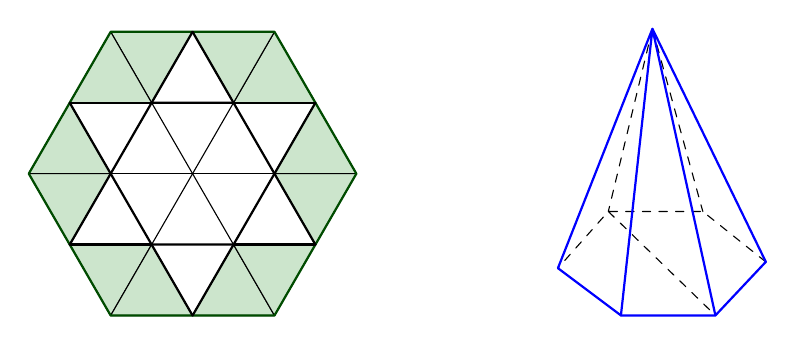
\begin{tikzpicture}[line cap=round, line join=round, >=stealth, font=\footnotesize, scale=0.8]
	\begin{scope}[shift={(0,0)}]
		\def\R{2.6} % Bán kính lục giác lớn bên ngoài
		\foreach \i in {1,...,6} {
			\coordinate (O\i) at ({60*\i-60}:\R);
		}
		\coordinate (Center) at (0,0);
		\foreach \i in {1,...,6} {
			\coordinate (I\i) at ({60*\i-60}:{\R/2});
		}
		\foreach \i in {1,...,6} {
			\coordinate (M\i) at ({60*\i-30}:{\R*cos(30)}); 
		}
		\foreach \i in {1,...,6} {
			\pgfmathtruncatemacro{\next}{mod(\i,6)+1}
			\fill[green!50!black!20, draw=black, thin] (O\i) -- (M\i) -- (I\i) -- cycle;
			\fill[green!50!black!20, draw=black, thin] (O\next) -- (M\i) -- (I\next) -- cycle;
		}
		\draw[thick, green!30!black] (O1) -- (O2) -- (O3) -- (O4) -- (O5) -- (O6) -- cycle;
		\draw[thick] (I1) -- (I2) -- (I3) -- (I4) -- (I5) -- (I6) -- cycle;
		\foreach \i in {1,...,6} {
			\draw[thin] (Center) -- (I\i);
		}
		\foreach \i in {1,...,6} {
			\pgfmathtruncatemacro{\next}{mod(\i,6)+1}
			\draw[thick] (I\i) -- (M\i);
			\draw[thick] (I\next) -- (M\i);
		}
	\end{scope}
	\begin{scope}[shift={(5.8,-1.5)}]
		\coordinate (A1) at (0,0);
		\coordinate (A2) at (1.0,-0.75);
		\coordinate (A3) at (2.5,-0.75);
		\coordinate (A4) at (3.3,0.1);
		\coordinate (A5) at (2.3,0.9);
		\coordinate (A6) at (0.8,0.9);
		\coordinate (S) at (1.5,3.8);
		\draw[dashed,thin] (A4)--(A5)--(A6)--(A1) (A6)--(A3) (S)--(A6) (S)--(A5);
		\draw[thick,blue] (A1)--(A2)--(A3)--(A4);
		\draw[thick,blue] (A4)--(S)--(A1) (A3)--(S)--(A2);
	\end{scope}
	
\end{tikzpicture}
	\end{center}
	\par \shortans[oly]{624}
	\loigiai{
	Gọi $O$ là tâm của hình lục giác đều.\\
	Gọi $x$, $y$ lần lượt là cạnh đáy, cạnh bên của hình chóp lục giác đều thu được.
	\begin{center}
		\begin{tikzpicture}[line cap=round, line join=round, >=stealth, font=\footnotesize, scale=0.8]
			\begin{scope}[shift={(0,0)}]
				\path (0,0) coordinate (O);
				\def\R{2.6} % Bán kính lục giác lớn bên ngoài
				\foreach \i in {1,...,6} {
					\coordinate (O\i) at ({60*\i-60}:\R);
				}
				\coordinate (Center) at (0,0);
				\foreach \i in {1,...,6} {
					\coordinate (I\i) at ({60*\i-60}:{\R/2});
				}
				\foreach \i in {1,...,6} {
					\coordinate (M\i) at ({60*\i-30}:{\R*cos(30)}); 
				}
				\foreach \i in {1,...,6} {
					\pgfmathtruncatemacro{\next}{mod(\i,6)+1}
					\fill[green!50!black!20, draw=black, thin] (O\i) -- (M\i) -- (I\i) -- cycle;
					\fill[green!50!black!20, draw=black, thin] (O\next) -- (M\i) -- (I\next) -- cycle;
				}
				\draw[thick, green!30!black] (O1) -- (O2) -- (O3) -- (O4) -- (O5) -- (O6) -- cycle;
				\draw[thick] (I1) -- (I2)-- (I3)node[below,midway,sloped]{$x$}-- (I4) -- (I5) -- (I6) -- cycle;
				\foreach \i in {1,...,6} {
					\draw[thin] (Center) -- (I\i);
				}
				\foreach \i in {1,...,6} {
					\pgfmathtruncatemacro{\next}{mod(\i,6)+1}
					\draw[thick] (I\i) -- (M\i);
					\draw[thick] (I\next) -- (M\i);
				}
				\path ($(I1)!(M1)!(I2)$) coordinate (H);
				\foreach \x/\goc in {O/-90,H/180}
				\fill (\x) node[shift={(\goc:8pt)},font = \footnotesize]{$\x$} circle (1pt);
				\fill (O1) circle(1.2pt) node[right]{$A$}
				(O2) circle(1.2pt) node[above]{$B$}
				(M1) circle(1.2pt) node[right]{$P$}
				(I1) circle(1.2pt) node[below right]{$M$}
				(I2) circle(1.2pt) node[above left]{$N$}
				;
				
				\draw (I1)--(M1)node[below,midway,sloped]{$y$} (M1)--(H);
				\draw pic[draw,angle radius=1.5mm]{right angle=I1--H--M1};
			\end{scope}
			\begin{scope}[shift={(5.8,-1.5)}]
				\coordinate (A1) at (0,0);
				\coordinate (A2) at (1.0,-0.75);
				\coordinate (A3) at (2.5,-0.75);
				\coordinate (A4) at (3.3,0.1);
				\coordinate (A5) at (2.3,0.9);
				\coordinate (A6) at (0.8,0.9);
				\coordinate (S) at (1.5,3.8);
				\draw[dashed,thin] (A4)--(A5)--(A6)--(A1) (A6)--(A3) (S)--(A6) (S)--(A5);
				\draw[thick,blue] (A1)--(A2)node[below,midway,sloped]{$x$}--(A3)--(A4);
				\draw[thick,blue] (A4)--(S)--(A1)node[above,midway,sloped]{$y$} (A3)--(S)--(A2);
			\end{scope}
			
		\end{tikzpicture}
	\end{center}
	Diện tích đáy của hình chóp bằng $6 \cdot \dfrac{x^2\sqrt{3}}{4}=\dfrac{3x^2\sqrt{3}}{2}$.\\
		Ta có $OP=20 \cdot \dfrac{\sqrt{3}}{2}=10\sqrt{3} \Rightarrow PH= 10\sqrt{3}-\dfrac{x\sqrt{3}}{2}$.\\
	Suy ra $y^2=\dfrac{3(20-x)^2}{4}+\dfrac{x^2}{4}=x^2-30x+300$.\\
	Chiều cao hình chóp là $h=\sqrt{y^2-x^2}=\sqrt{300-30x}$.\\
	Thể tích hình chóp là $V=\dfrac{1}{3} \cdot \dfrac{3x^2\sqrt{3}}{2} \cdot \sqrt{300-30x}=\dfrac{3\sqrt{10}}{2}\sqrt{x^4(10-x)}$.\\
	Hàm số $f(x)=10x^4-x^5$ có bảng biến thiên trên khoảng $(0;10)$ như sau
		\begin{center}
			
\begin{tikzpicture}
				\tkzTabInit[lgt=1.5,espcl=2.5,deltacl=0.5]{$x$/1,$f'(x)$/1,$f(x)$/2}{$0$,$8$,$10$}
				\tkzTabLine{,+,0,-,}
				\tkzTabVar{-/$0$,+/$ $, -/$0$}
			\end{tikzpicture}
		\end{center}
	Thể tích khối chóp thu được lớn nhất khi $x=8$. Khi đó $PH=6\sqrt{3}$.\\
	Khi đó diện tích toàn phần của hình chóp là $\dfrac{3 \cdot 8^2\sqrt{3}}{2}+6 \cdot \dfrac{1}{2} \cdot 6\sqrt{3} \cdot 8=240\sqrt{3}$.\\
	Diện tích của tấm bìa là $S=6\cdot \dfrac{20^2\sqrt{3}}{4}=600\sqrt{3}$.\\
	Vậy diện tích bạn Bình cắt đi là $600\sqrt{3}-240\sqrt{3}=360\sqrt{3}\approx 624$ (đvdt).
	}
\end{ex}

\begin{ex}%[1D2V3-8]
	Để tiết kiệm năng lượng, một công ty điện lực đề xuất bán điện sinh hoạt cho người dân theo hình thức lũy tiến (bậc thang) như sau: Mỗi bậc gồm $40$ số; bậc $1$ từ số thứ $1$ đến số thứ $40$, bậc $2$ từ số thứ $41$ đến số thứ $80$, bậc $3$ từ số thứ $81$ đến số thứ $120$,\ldots. Bậc $1$ có giá là $1\,900$ đồng/$1$ số, giá của mỗi số ở bậc thứ $n+1$ tăng so với giá của mỗi số ở bậc thứ $n$ là $5\%$. Gia đình ông A sử dụng hết $487$ số trong tháng $3$ thì ông A phải nộp bao nhiêu nghìn đồng (\textit{không làm tròn kết quả các phép tính trung gian, chỉ làm tròn kết quả cuối cùng đến hàng đơn vị})?
	\par \shortans[oly]{1234}
	\loigiai{
		Gọi $u_1$ là số tiền phải trả cho $40$ số điện đầu tiên.\\
		Khi đó $u_1=40 \cdot 1{,}9=76$ (nghìn đồng).\\
		Và $u_2$ là số tiền phải trả cho các số điện từ $41$ đến $80$, hay $u_2=u_1(1+0{,}05)$.\\
		Ta có $u_{12}$ là số tiền phải trả cho các số điện từ $441$ đến $480$, hay $u_{12} = u_1(1+0{,}05)^{11}$.\\
		Số tiền phải trả cho $480$ số điện đầu tiên là $S_1=u_1 \cdot \dfrac{1-(1+0{,}05)^{12}}{1-(1+0{,}05)}$.\\
		Số tiền phí trả cho các số điện từ $481$ đến $487$ là $S_2=7 \cdot 1{,}9(1+0{,}05)^{12}$.\\
		Vậy tháng $1$ gia đình ông A phải trả số tiền là $S=S_1+S_2\approx 1\,234$ (nghìn đồng).
	}
\end{ex}

\Closesolutionfile{ans}


%\begin{center}
%	\textbf{PHẦN 4 - Phần tự luận}
%\end{center}
%\setcounter{ex}{0}
%
%\Opensolutionfile{ans}[ans-KQ]
%%-----Câu 1
%\begin{ex}%[ID]%[KNTT - Lớp 10 - Ôn tập giữa học kì 1 - Đề 1]%[Dương Văn Đức]
%	
%	\loigiai{
%	}
%\end{ex}
%
%\Closesolutionfile{ans}

